\documentclass[12pt,a4paper]{report}

\usepackage[utf8x]{inputenc}
\usepackage{amsmath}
\usepackage{amsfonts}
\usepackage{amssymb}
\usepackage{graphicx}
\usepackage{enumitem}
\usepackage{pgf}
\usepackage{tikz}
\usepackage{calrsfs}
\usepackage{algpseudocode}
\usetikzlibrary{arrows,automata,calc, positioning}

\begin{document}

\begin{titlepage}
	\centering
	{\scshape\LARGE Universidad Autónoma de México \par}
	\vspace{1cm}
	{\scshape\Large Computación Distribuida\par}
	\vspace{1.5cm}
	{\huge\bfseries Tarea I\par}
	\vspace{.5cm}
	{\Large\itshape Edgar Quiroz Castañeda \par}
    \vspace{.5cm}
	{\Large\itshape Jerónimo Almeida Rodríguez \par}
	\vfill
	 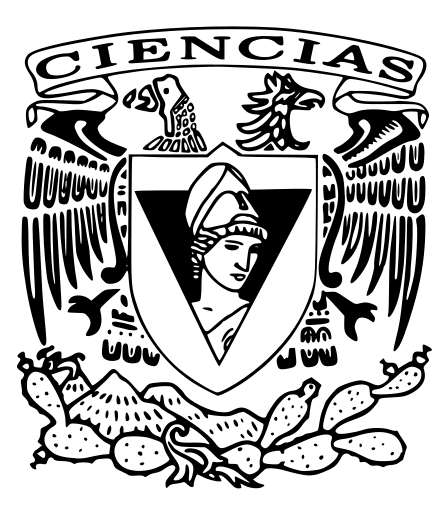
\includegraphics[width=0.5\textwidth]{escudo_f-ciencias.png}
	\vfill

% Bottom of the page
	{\large Jueves 23 de Agosto del 2018 \par}
\end{titlepage}

\pagebreak
\setlength{\voffset}{-0.75in}
\setlength{\headsep}{5pt}

\newcommand{\ed}[2]{(#1) edge (#2)}
\newcommand{\eee}[4]{\path [->,draw,thin] ($ (#1) !.5! (#2)$) -- ($ (#3) !.5! (#4) $);}


\begin{enumerate}
		%Ejercicio 1
		\item {
		Dada la siguiente gráfica $\mathcal{O}$, propón una tarea distribuida
		$T=\langle \mathcal{I}, \mathcal{O}, \Delta \rangle$ con salida $\mathcal{O}$.
		Describe el significado de todas las configuraciones iniciales en $T$
		utilizando alguna situación de la vida real, como los ejemplos con Alice y
		Bob vistos en clase y también describe a $\Delta$.\\
		\begin{center}
		  \begin{tikzpicture}[-,>=stealth',auto, node distance = 2.8cm,
				shorten > = 1pt, semithick, state/.style = {circle, fill=#1,
				draw=black!, inner sep=1mm, text=black}, state/.default = white]

			 \tikzstyle{every state}=[fill=white,draw=black!,text=black]

		  	 \node (AO0) [state]                      {$(A,0)$};%E
		  	 \node (BO0) [state=gray, right of=AO0] {$(B,0)$};%F
		     \node (BO3) [state=gray, below of=AO0]   {$(B,\frac{1}{3})$};%G
		  	 \node (AO2) [state, below of=BO3]        {$(A,\frac{2}{3})$};%H
		  	 \node (BO1) [state=gray, below of=AO2]   {$(B,1)$};%I
		   	 \node (AO3) [state, below of=BO0]        {$(A,\frac{1}{3})$};%J
		  	 \node (BO2) [state=gray, below of=AO3]   {$(B,\frac{2}{3})$};%K
		  	 \node (AO1) [state, below of=BO2]        {$(A,1)$};%L

		  	 \path  \ed{AO0}{BO0}
					\ed{AO0}{BO3}
					\ed{BO3}{AO2}
					\ed{AO2}{BO1}
					\ed{BO0}{AO3}
					\ed{AO3}{BO2}
					\ed{BO2}{AO1}
					(AO1) edge node {$\mathcal{O}$} (BO1);

		  \end{tikzpicture}
		\end{center}

		La tarea que proponemos es la siguiente: \\

		El Dr. Alfaro es el director de la planta nuclear del estado, pero necesita
		más	barras de uranio para que la planta pueda seguir trabajando, así que
		intenta contactar a la Dra. Benitez para comprarle uranio del que produce en
		su laboratorio. Por	azares del destino, la red local de comunicación se cayó,
		así que para comunicarse cada uno envía un mensajero.\\
		 El problema es que el cartel de los $\mathbb{N}$ está planeando robar el
		dinero, el uranio o ambos. Si capturan a los mensajeros podrán saber dónde
		se va a hacer la compra. Por esto mismo de la inseguridad, ninguna de las dos
		partes está segura de querer hacer el trato. Así que, dependiendo de la
		urgencia que tengan de cerrar el trato enviarán al mensajero para intentar
		convencer al otro de cerrar el trato o de no arriesgarse innecesariamente.\\
		 El doctor y la doctora saben que si los mensajeros son hábiles podrán
		escabullirse de los mafiosos, pero tienen la certeza de que si uno es
		capturado, entonces los mafiosos estarán demasiado ocupados con el cómo para
		intentar capturar al otro mensajero.\\\\
		$\mathcal{I}:=$ En la gráfica de entrada, consideramos los siguientes valores:
		(1) Si el Dr. Alfaro está dispuesto a comprar, (0) si no. (1) Si la doctora
		Benitez está dispuesta a vender, (0) si no.\\
		$\mathcal{O}:=$ Para la gráfica de salida, consideramos los siguientes
		valores: (0) Si el trato se cancela, (1) si ambos deciden cerrar el trato y 
		$\dfrac{1}{3} \lor \dfrac{2}{3}$ si están en desacuerdo y alguno de los
		mensajeros fue capturado.\\
		$\Delta:=$ Si ambos consideran que hacer la compra es de suma importacia,
		entonces ambos intentarán cerrar el trato. También, si consideran que	es
		demasiado riesgoso salir a cerrar el trato, entonces no lo harán. Por otro
		lado, si están en desacuerdo intentarán llegar a un compromiso dando mayor
		peso al otro lado del trato. Finalmente, si un mensajero es capturado, la
		parte receptora se adherirá a su decisión sin importar las consecuencias.\\
		Por ejemplo, la arista (0)-(1) en $\mathcal{I}$ significa que A no quiere
		comprar pero que B sí quiere vender. Entonces, una salida 
		$(\frac{2}{3})-(\frac{1}{3})$ significa que B va a pagar 1/3 de lo que
		normalmente pagaría para poder resolver el problema. Y B, como sabe que A no
		quiere vender, entonces va a comprarle 2/3 de lo que había ofrecido 
		originalmente.\\
		De igual manera, si hay problemas de comunicación y no saben que quiere el
		otro, entonces asumirán su parte del trato. Así, con (0)-(1), una salida 0 1/3
		significaría que a B nunca le llegó el mensaje sobre la oferta de A, y como A
		sabe que B no quiere comprar, sólo va a darle el 1/3 del uranio. También, el
		(1/3) de diferencia es el margen de perdida aceptable en caso que la
		comunicación falle.

		\begin{tikzpicture}[-,>=stealth',auto,
		node distance = 2.8cm,
		    shorten > = 1pt, semithick,
		 state/.style = {circle, fill=#1, draw=black!,
		                 inner sep=1mm, text=black},
		 state/.default = white]

		  \tikzstyle{every state}=[fill=white,draw=black!,text=black]

		  \node (AI0) [state]                      {$(A,0)$};%A
		  \node (BI0) [state=gray, right of =AI0]   {$(B,0)$};%B
		  \node (AI1) [state, below of=BI0]        {$(A,1)$};%C
		  \node (BI1) [state=gray, below of=AI0]   {$(B,1)$};%D
		  \node (AO0) [state, above right = 3cm and 3cm of BI0]  {$(A,0)$};%E
		  \node (BO0) [state=gray, right of=AO0]   {$(B,0)$};%F
		  \node (BO3) [state=gray, below of=AO0]   {$(B,\frac{1}{3})$};%G
		  \node (AO2) [state, below of=BO3]        {$(A,\frac{2}{3})$};%H
		  \node (BO1) [state=gray, below of=AO2]   {$(B,1)$};%I
		  \node (AO3) [state, below of=BO0]        {$(A,\frac{1}{3})$};%J
		  \node (BO2) [state=gray, below of=AO3]   {$(B,\frac{2}{3})$};%K
		  \node (AO1) [state, below of=BO2]        {$(A,1)$};%L

		  \path \ed{AI0}{BI0}
			    \ed{BI0}{AI1}
			    \ed{AI0}{BI1}
			    (AI1) edge node {$\mathcal{I}$} (BI1)
				\ed{AO0}{BO0}
				\ed{AO0}{BO3}
				\ed{BO3}{AO2}
				\ed{AO2}{BO1}
				\ed{BO0}{AO3}
				\ed{AO3}{BO2}
				\ed{BO2}{AO1}
				(AO1) edge node {$\mathcal{O}$} (BO1);

		  \eee{AI1}{BI1}{BO1}{AO1}
		  \eee{AI0}{BI0}{AO0}{BO0}
		  \eee{AI0}{BI1}{AO0}{BO3}
		  \eee{AI0}{BI1}{BO3}{AO2}
		  \eee{AI0}{BI1}{AO2}{BO1}
		  \eee{AI0}{BI1}{AO0}{BO3}
		  \eee{AI1}{BI0}{AO3}{BO0}
		  \eee{AI1}{BI0}{BO2}{AO3}
		  \eee{AI1}{BI0}{AO1}{BO2}

		\end{tikzpicture}
	}
	\item {
	Dado el problema del inciso anterior, propón un algoritmo en el modelo de
	comunicación siguiente y demuestra que es correcto.\\\\
		\begin{equation*}
			\mathcal{M} = \{A \leftrightarrow B, A \rightarrow B, A \leftarrow B \}
		\end{equation*}\\
	El algoritmo propuesto es el siguiente para ambos procesos.\\
		\begin{algorithmic}[1]
			\Require $init \in \{0, 1\}$
			\Function{$\frac{1}{3}-AproximateAgreement$}{$init$}
				\State $send(init)$
				\State $x \gets receive()$
				\If{$x \ne null$}
					\State \Return $\frac{init + 2x}{3}$
				\Else
					\State \Return $init$
				\EndIf
			\EndFunction
		\end{algorithmic}

	Veamos que es correcto, es decir que los estados finales son válidos.\\\\

	Primero, supongamos, sin perder generalidad, que $init_A = init_B = v$ .\\
	Pueden pasar dos cosas, que haya comunicación perfecta o que se pierda uno
	de los mensajes.\\
	Si hay comunicación perfecta, entonces los dos procesos ejecutan la línea 5,
	y se tiene que los dos procesos regresan $\frac{v + 2v}{3} = \frac{3v}{3} = v$.\\
	Si alguno de los mensajes se pierde, supongamos sin perder generalidad que a $A$
	no le llega el mensaje.\\
	Entonces, $A$ ejecuta la línea 7 y regresa $init_A = v$.\\
	El proceso $B$ sí recibe el mensaje, por lo que ejecuta la línea 5 y regresa
	$\frac{init_A + 2 (init_B)}{3} = \frac{v + 2v}{3} = \frac{3v}{3} = v$.\\
	Entonces todos los casos los dos procesos regresan $v$, que es bien 1 o 0,
	ambos estados finales válidos.\\
	Entonces, si las entradas son iguales, el algoritmo produce etados finales válidos.\\\\

	Luego, supongamos que $init_A \ne init_B$.\\
	Si hay comunicación perfecta, entonces ambos procesos ejecutan la línea 5.\\
	Si $init_A = 1$ y $init_B = 0$, entonces el proceso $A$ regresa
	$\frac{init_A + 2(init_B)}{3} = \frac{1}{3}$ y el proceso $B$ regresa
	$\frac{init_B + 2(init_A)}{3} = \frac{2}{3}$, que es un estado final válido.\\
	Si $init_A = 0$ y $init_B = 1$, entonces el proceso $A$ regresa
	$\frac{init_A + 2(init_B)}{3} = \frac{2}{3}$ y el proceso $B$ regresa
	$\frac{init_B + 2(init_A)}{3} = \frac{1}{3}$, que también es un estado final válido.\\
	Si alguno de los mensajes se pierde, supongamos sin perder generalidad que a $A$
	no le llega el mensaje.\\
	Entonces $A$ ejecuta la línea 5 y regresa $init_A$.\\
	El proceso $B$ sí recibe el mensaje, por lo que ejecuta la línea 5 y regresa
	$\frac{init_A + 2 (init_B)}{3}$.\\
	Si $init_A = 1$ y $init_B = 0$, entonces el proceso $A$ regresa $init_A = 1$
	y el proceso $B$ regresa $\frac{init_B + 2(init_A)}{3} = \frac{2}{3}$,
	que es un estado final válido.\\
	Si $init_A = 0$ y $init_B = 1$, entonces el proceso $A$ regresa $init_A = 0$
	y el proceso $B$ regresa $\frac{init_B + 2(init_A)}{3} = \frac{1}{3}$,
	que también es un estado final válido.\\
	Entonces, si las entradas son diferentes, el algoritmo produce etados finales
	válidos.\\\\
	Entonces, con todas las diferentes entradas y posibles errores de comunicación,
	el algoritmo produce estados finales válidos.\\
	Por lo tanto, el algoritmo es correcto.\\\\
	}
\end{enumerate}
\end{document}
